\documentclass{article}
\usepackage{graphicx}
\usepackage{ragged2e}
\usepackage{hyperref}
\usepackage{tex4ebook}
\usepackage{ifpdf}
\usepackage{float}
\usepackage{titlesec}
\usepackage{listings}
\usepackage{xcolor}

\usepackage{variables}
\titleformat{\section}[block]{\normalfont\Large\bfseries}{\thesection}{1em}{}
\titlespacing*{\section}{0pt}{\baselineskip}{\baselineskip}

\lstset{
  basicstyle=\ttfamily,
  escapeinside=||
}

\setlength{\parskip}{\baselineskip}%
\title{
  
\includegraphics[width=5cm]{Images/Logo.png}\\
  \normalsize Department of Electrical and Computer Engineering\\
  ENEL 453: Digital System Design
}

\date{\semester}

\makeatletter
\renewcommand{\maketitle}{%
  \begin{center}
    {\@title}
    \vspace{1cm} % Space between title and date, adjust as needed
    {\@date}
  \end{center}
}
\makeatother

\begin{document}
\centering

\maketitle
\large Lab 1: Correction \\
\large Addendum 

\RaggedRight
\section{CDMA2000}
In the initial lab document instructions were provided for changing the initial state of the CRC in order to calculate the CDMA2000 CRC which requires that the register have an initial condition of 0xFFFF. However if you follow just the instructions provided you will arrive at the following output for your CRC simulation:
\begin{verbatim}
    Original Message: Hello, CRC!
    Calculated CRC (Hex): 73e8
\end{verbatim}
However, this is incorrect as the value should have been: 0x84C5. If you follow along performing the steps one by one, you'll notice the following. 

\begin{itemize}
    \item Using the following online crc calculator \url{http://www.sunshine2k.de/coding/javascript/crc/crc_js.html} you can verify the initial calculated CRC for XMODEM. 
    \item If we then change the polynomial but keep the initial conditions as zero we calculate 0x1c99. This matches for both the simulation and for the online calculators. 
        \begin{verbatim}
            Original Message: Hello, CRC!
            Calculated CRC (Hex): 1c99
        \end{verbatim}  
    \item If we then change the initial conditions to 0xFFFF in this new calculator we get 0x84C5 which matches the original online calculator. This allows us to limit our investigation of the bug down to just the code relating to the initial values. The initial value instructions were in error. So you should change the reset value for CRC\_REG back to:
    \begin{verbatim}
        CRC_REG <= 16'h0000;  // Reset the CRC Register to 0
    \end{verbatim}
    and change the fill value back to zero in the read mode like this:
    \begin{verbatim}
        // Shift the CRC Register Left by One Bit
        CRC_REG <= {CRC_REG[14:0], 1'b0}; 
    \end{verbatim}
\end{itemize}

There are a few mistakes that combine to produce the incorrect value. The following is how to change the init value to correctly produce the CDMA2000 CRC.

\subsection{Modify the Initial Value}
CRC Initial values are a value which the intitial bits of the message are XOR'd by to produce more reliable behavior. CDMA2000 has an init value of 0xFFFF, this protects it from cases where the data value is zeroed out, which would produce incorrectly valid CRCs for XMODEM. You can see this by feeding in all zero values to the CRC calculator.

Initially when making this lab I set the CRC reg to the initial value and assumed incorrectly that this would result in the correct value regardless of the init used for the specific CRC. This was wrong, and is a simplification that only works for zero as the init value. Some additional hardware is required to produce the correct value for other init values. 

\subsubsection{Add a new CRC Init Register}
\begin{verbatim}
    logic [15:0] CRC_INIT;
\end{verbatim}
Add this line immediately after the declaration for the original CRC register. 

\subsubsection{Initialize the CRC Init Register to the Appropriate Value}
\begin{verbatim}
    CRC_INIT <= 16'hFFFF;
\end{verbatim}
Add this line in the reset code to set the CRC Init register when the module is reset. Also add it to the READ\_MODE code to reset the initial value after the module has been used once. 

\subsubsection{Apply the initial value Register}
\begin{verbatim}
    CRC_REG[0] <= DATA_IN ^ CRC_REG[15] ^ CRC_INIT[15];
\end{verbatim}
Modify your CRC\_REG value to include an XOR with the CRC\_INIT register. For this line we're just going to apply the MSB of the CRC init register. We'll add another line to shift the data over so that all values in the register get applied.

\subsubsection{Shift the initial value Register}
\begin{verbatim}
    CRC_INIT <= {CRC_INIT[14:0], 1'b0}; 
\end{verbatim}
This shifts over the register values one bit at a time and in-fills zeros into the CRC init register. This means that the first two bytes of the CRC will have their values altered as they enter the shift register, but afterwards they will behave as they did in the original code. 

\section{Verification}
This where I fell down in the initial lab where I didn't fully verify my outputs against a known good output. To compensate for that I can now properly verify the implemented CRC init register by checking various different init values and comparing them to the online calculator. 

\centering{Checking 0xF0F0}
\begin{figure}[H]
    \centering
    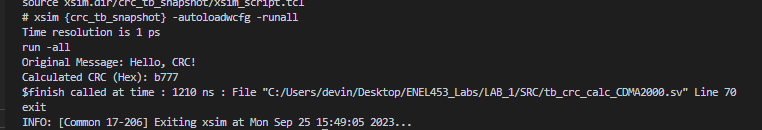
\includegraphics[width = 10cm]{Lab_1/Lab_1_Correction/Images/0F0F_verification.png}
    \caption{Simulation Results}
    \label{fig:simulationresult}
\end{figure}
\begin{figure}[H]
    \centering
    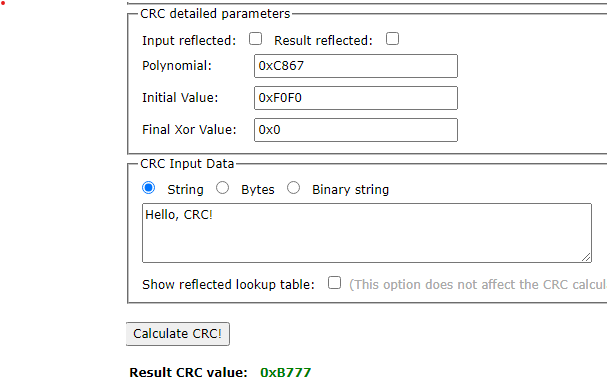
\includegraphics[width = 10cm]{Lab_1/Lab_1_Correction/Images/0F0F_verificationsite.png}
    \caption{Online Calculator}
    \label{fig:online_calc}
\end{figure}

I then asked a random number generator to generate me 3 more possible tests. It decided on EE73, 5A48, and E781. 

\begin{verbatim}
    Original Message: Hello, CRC!
    Calculated CRC (Hex): bf45
\end{verbatim}

\begin{verbatim}
    Result CRC value: 0xBF45
\end{verbatim}

\begin{verbatim}
    Original Message: Hello, CRC!
    Calculated CRC (Hex): dda1
\end{verbatim}

\begin{verbatim}
    Result CRC value: 0xDDA1
\end{verbatim}

\begin{verbatim}
    Original Message: Hello, CRC!
    Calculated CRC (Hex): d0d5
\end{verbatim}

\begin{verbatim}
    Result CRC value: 0xD0D5
\end{verbatim}

\RaggedRight
Given the outputs for each of these confirms with the tools this would suggest that it is very likely that the implementation is now fully correct. If moving this to silicon however, we would likely want to mirror our implementation in another more friendly language and verify across a number of randomized test inputs that the results match.
\end{document}

